\documentclass[t,aspectratio=169]{beamer}

\usepackage{bm}
\usepackage{soul}
\usepackage{tikz}
\usepackage{tikz-3dplot}
\usepackage{amsmath}
\usepackage{amsfonts}
\usepackage{amssymb}
%\usepackage{physics}
%\usepackage{graphicx}
\usepackage{multicol}
\usepackage[utf8]{inputenc}
\usepackage[magyar]{babel}

\usetikzlibrary{calc,3d,decorations.pathmorphing,decorations.pathreplacing,decorations.markings,snakes,arrows.meta,calc,patterns
}
\tikzset{snake it/.style={decorate, decoration=snake}}
% \usetheme{Madrid}
% \usecolortheme{whale}

%\usepackage{hyperref}
\hypersetup{
    colorlinks=true,
    linkcolor=blue,
    filecolor=magenta,      
    urlcolor=cyan,
    pdftitle={(KTXFI1EBNF) Physics I. Lecture},
}

% ----------------------------------------------------------------------------------------------------------------------------------------

\title{\includegraphics[width=45pt]{oepecsetlogo.png}\\(KTXFI1EBNF) Physics I. Lecture}

\author{Dr.~Gábor FACSKÓ, PhD\\\tiny Assistant Professor / Senior Research Fellow\\\textit{facsko.gabor@uni-obuda.hu}}

\institute{\Tiny Óbuda University, Faculty of Electrical Engineering, 1084 Budapest, Tavaszmező u. 17.\\Wigner Research Centre for Physics, Department of Space Physics and Space Technology, 1121 Budapest, Konkoly-Thege Miklós út 29–33.\\ \url{https://wigner.hu/~facsko.gabor}}

\date{March~23,~2026}

\logo{\includegraphics[height=0.9 true cm]{kekcsik.png}}

% ----------------------------------------------------------------------------------------------------------------------------------------

\begin{document}

\frame{\titlepage}

% ----------------------------------------------------------------------------------------------------------------------------------------

\begin{frame}
\frametitle{Current Updates and Issues}
\begin{itemize}
\setlength{\parskip}{0pt}
\setlength{\itemsep}{4pt}
\item Thank you for submitting your first homework assignment. I will grade the papers and provide the solutions soon.
\item Proposed midterm exam date: \textbf{May~11,~2026}. Retake: \textbf{May~18,~2026}.
\end{itemize}
\end{frame}

% ----------------------------------------------------------------------------------------------------------------------------------------

\begin{frame}[fragile,squeeze,allowframebreaks]
\frametitle{Where are we?}
\begin{enumerate}
\setlength{\parskip}{0pt}
\setlength{\itemsep}{0pt}
\item \textbf{Mechanics I.:} Newton’s laws, equation of motion (review). Momentum. General concept of mechanical work, work theorem. Forms of mechanical energy.
\item \textbf{Mechanics II.:} Weight force, gravitational force, gravitational field. Work of the gravitational force. Conservative force field. Dissipative force field. Mechanical power.
\item \textbf{Mechanics of Rigid Bodies I.} Concept of a rigid body. Forces acting on a rigid body. Motion of a rigid body. Concept of the centre of mass. Location of the centre of mass. Torque. Angular momentum. Energy of a rotating rigid body, angular momentum of a rotating rigid body, Steiner’s theorem.
\item \textbf{Mechanics of Rigid Bodies II.} Principal theorems of rigid body motion; conservation laws. Collisions.
\item \textbf{Oscillations I.} Dynamic condition of harmonic oscillatory motion. Differential equation of harmonic undamped oscillatory motion.
\pagebreak
\item \textbf{Oscillations II.} Superposition of oscillations. Decomposition of oscillations into components. Damped oscillations. Forced oscillations, resonance. Coupled oscillations.
\item \textbf{Wave phenomena:} Reflection of waves, refraction of waves, diffraction of waves. Huygens–Fresnel principle. Interference of waves. Polarization of waves.
\item \textbf{Elements of acoustics:} Basics of acoustics. Fundamental concepts. Doppler effect. Sound intensity, loudness according to Weber–Fechner’s law.
\item \textbf{Thermodynamics I:} Temperature scales, thermal expansion, thermometers. State variables, ideal gas, state changes, ideal gas equation of state, Boyle’s law, Gay-Lussac’s laws, universal (combined) gas law, heat, specific heat, molar heat, heat capacity.
\item \textbf{Thermodynamics II:} Expansion work, internal energy, the first law of thermodynamics, forms of the first law in different state changes.
\pagebreak
\vskip -10 pt
\item \textbf{Thermodynamics III:} \textit{Cyclic processes, Carnot cycle, Carnot’s theorem, reduced heat, entropy, the second law of thermodynamics.}
\item \textbf{Thermodynamics IV:} Kinetic theory of gases, molecular thermodynamics. Distributions, distribution functions. Elementary statistics.
\item \textbf{Electrostatics I.:} Electric charge: Fundamental electrical phenomena, electric charge and matter, Coulomb’s law (force between two point charges, unit of electric charge, permittivity of vacuum).
\item \textbf{Electrostatics II.:} The electric field: The electrostatic field (electric field strength, electric field lines). Determination of electric field strength. Gauss’s law (flux of the electric field). Electric field of a point charge.
\pagebreak
\item \textbf{Electrostatics III.:} Electrostatic potential: Work of the electric field (work done in an electric field). Electric potential (electrostatic potential). Electric potential difference, voltage. Electric potential of charge systems at small and large distances. Electrostatic energy.
\item \textbf{Elements of physical or wave optics.} Branches of optics. Light interference, light diffraction, diffraction through a slit, optical grating, light polarization. Light as an electromagnetic wave: Poynting vector. Optical instruments.
\end{enumerate}
\end{frame}

% ----------------------------------------------------------------------------------------------------------------------------------------

\begin{frame}[fragile,squeeze,allowframebreaks]
\frametitle{Thermodynamic cycles}
\begin{itemize}
\item  \textbf{Definition (thermodynamic cycle):} During the cycle, the substance returns to the initial state after successive processes or change in state.
\begin{columns}
\begin{column}{0.4\textwidth}
  \vfill
\begin{center}
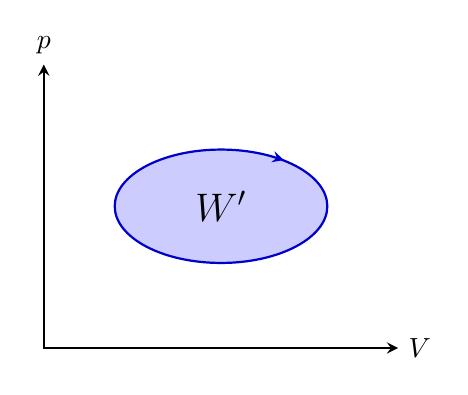
\begin{tikzpicture}[scale=0.9,line cap=round, line join=round, >=stealth]
    % Tengelyek rajzolása feketével, nyilakkal
    \draw[->, thick, black] (0,0) -- (5,0) node[right] {$V$};
    \draw[->, thick, black] (0,0) -- (0,4) node[above] {$p$};

    % Az ovális alapzat (világoskék kitöltés, sötétkék keret)
    % A 'postaction' segítségével tesszük rá az óramutató járásával megegyező nyílfejet
    \filldraw[fill=blue!20, draw=blue!80!black, thick, 
              postaction={decorate, decoration={markings, mark=at position 0.15 with {\arrow{<}}}}] 
              (2.5,2) ellipse (1.5cm and 0.8cm);

    % A nagy fekete W' felirat az ovális közepén
              \node[black] at (2.5,2) {\Large $W'$};
\end{tikzpicture}
\end{center}
\end{column}
\begin{column}{0.4\textwidth}
\begin{itemize}
\item The area enclosed by the curve of the cycle on the $p-V$ state diagram represents the magnitude of the work obtained.
\item If the direction of the cycle changes $\implies$ the sign of the work changes $W' \to W$
\end{itemize}
\end{column}
\end{columns}

\pagebreak
\item \textbf{Definition (thermal efficiency of the cycle):}
    $$\eta = \frac{\text{The work done by the system}}{\text{Cold (absorbed) heat}} = \frac{W'}{Q_{absorbed}}$$
\item \textbf{Consequences:}
  $$\eta = \frac{Q_{absorbed} - Q_{released}}{Q_{absorbed}} = \frac{\sum Q}{Q_{absorbed}}$$

\pagebreak
\item \textbf{Carnot-cycle:} (Sadi Nicolas Leonard Carnot, 1796-1832)
\begin{columns}
\begin{column}{0.4\textwidth}
\vfill
\begin{center}
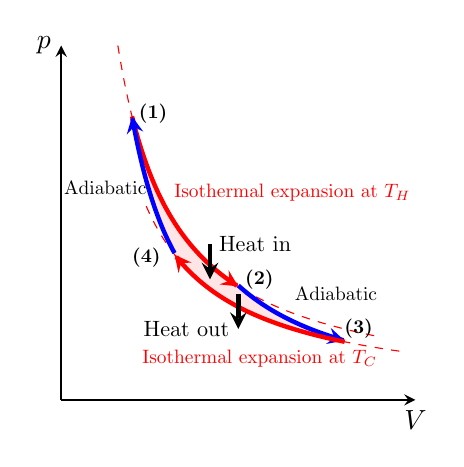
\begin{tikzpicture}[scale=0.9,>=stealth]
    % Tengelyek
    \draw[thick, ->] (0,0) -- (5,0) node[below] {$V$};
    \draw[thick, ->] (0,0) -- (0,5) node[left] {$p$};

    % Koordináták kiszámítása az illeszkedéshez
    % A: (1, 4), B: (2.5, 1.6) -> Izoterma (P=4/V)
    % B: (2.5, 1.6), C: (4, 0.82) -> Adiabata (P=k/V^1.4)
    % C: (4, 0.82), D: (1.6, 2.05) -> Izoterma (P=3.28/V)
    % D: (1.6, 2.05), A: (1, 4) -> Adiabata

    % Rózsaszín kitöltés
    \fill[pink!40] 
        plot[domain=1:2.5, samples=100] (\x, {4/\x}) -- 
        plot[domain=2.5:4, samples=100] (\x, {5.82/(\x^1.4)}) -- 
        plot[domain=4:1.6, samples=100] (\x, {3.28/\x}) -- 
        plot[domain=1.6:1, samples=100] (\x, {4/(\x^1.4)}) -- cycle;

    % Szaggatott vékony izotermák
    \draw[red, dashed, thin] plot[domain=0.8:4.5, samples=100] (\x, {4/\x});
    \draw[red, dashed, thin] plot[domain=1.2:4.8, samples=100] (\x, {3.28/\x});

    % 1. Izotermális tágulás (Vörös, vastag)
    \draw[red, ultra thick, ->] plot[domain=1:2.5, samples=100] (\x, {4/\x});
    \node[red, above right, scale=0.7] at (1.5, 2.7) {Isothermal expansion at $T_H$};
    \node[black, above right, scale=0.7] at (1.0, 3.8) {\textbf{(1)}};

    % 2. Adiabatikus tágulás (Kék, vastag)
    \draw[blue, ultra thick, ->] plot[domain=2.5:4, samples=100] (\x, {5.82/(\x^1.4)});
    \node[black, right, scale=0.7] at (3.2, 1.5) {Adiabatic};
    \node[black, right, scale=0.7] at (2.5, 1.7) {\textbf{(2)}};

    % 3. Izotermális összenyomás (Vörös, vastag)
    \draw[red, ultra thick, ->] plot[domain=4:1.6, samples=100] (\x, {3.28/\x});
    \node[red, below, scale=0.7] at (2.8, 0.8) {Isothermal expansion at $T_C$};
    \node[black, right, scale=0.7] at (3.9, 1.0) {\textbf{(3)}};

    % 4. Adiabatikus összenyomás (Kék, vastag)
    \draw[blue, ultra thick, ->] plot[domain=1.6:1, samples=100] (\x, {4/(\x^1.4)});
    \node[black, left, scale=0.7] at (1.3, 3) {Adiabatic};
    \node[black, left, scale=0.7] at (1.5, 2.0) {\textbf{(4)}};

    % Hőcsere nyilak (fekete, merőleges)
    \draw[black, ultra thick, ->] (2.1, 2.2) -- (2.1, 1.7) node[right, pos=0, scale=0.8] {Heat in};
    \draw[black, ultra thick, ->] (2.5, 1.5) -- (2.5, 1.0) node[left, pos=1, scale=0.8] {Heat out};
\end{tikzpicture}
\end{center}
\end{column}
\begin{column}{0.6\textwidth}
\begin{enumerate}
\item Isothermal: $W'_1 = Q_1 = \frac{m}{M} \cdot R \cdot T_H \ln \frac{V_B}{V_A}$
\item Adiabatic: $W'_2 = -c_V \cdot m \cdot (T_C - T_H) \quad Q = 0$
\item Isothermal: $W'_3 = Q_2 = \frac{m}{M} \cdot R \cdot T_C \ln \frac{V_D}{V_C}$
\item Adiabatic: $W'_4 = -c_V \cdot m \cdot (T_H - T_C) \quad Q = 0$
\end{enumerate}
$Q_1$ is absorbed heat, $Q_2$ is released heat, $T_{H}$ is the higher temperature, and $T_{C}$ is lower temperature. 
\end{column}
\end{columns}


\pagebreak
\item  $\eta_C = \frac{\sum_{i=1}^4 W'}{Q_{absorbed}} = \frac{\frac{m}{M} \cdot R \cdot T_H \ln \frac{V_B}{V_A} - c_V \cdot m \cdot (T_C - T_H) + \frac{m}{M} \cdot R \cdot T_C \ln \frac{V_D}{V_C} - c_V \cdot m \cdot (T_H - T_C)}{\frac{m}{M} \cdot R \cdot T_H \ln \frac{V_B}{V_A}}$ \

\item However, $T_H V_B^{\kappa-1} = T_C V_C^{\kappa-1}$ and $T_H V_A^{\kappa-1} = T_C V_D^{\kappa-1} \implies \frac{V_B}{V_A} = \frac{V_C}{V_D}$ $(*)$

$\eta_C = \frac{\sum_{1}^4 W'}{Q_{absorbed}} = \frac{\frac{m}{M} \cdot R \cdot T_H \ln \frac{V_B}{V_A} + \frac{m}{M} \cdot R \cdot T_C \ln \frac{V_D}{V_C}}{\frac{m}{M} \cdot R \cdot T_H \ln \frac{V_B}{V_A}} = \frac{\frac{m}{M} \cdot R \cdot T_H \ln \frac{V_B}{V_A} + \frac{m}{M} \cdot R \cdot T_C \ln \frac{V_A}{V_B}}{\frac{m}{M} \cdot R \cdot T_H \ln \frac{V_B}{V_A}} = \frac{T_H - T_C}{T_H}$

\pagebreak
\item The second law of thermodynamics
\begin{itemize}
\item \textbf{Rudolf Clausius’ definition (1822 – 1888):} Heat energy does not spontaneously flow from a lower temperature body to a higher temperature body without any other changes occurring.
\item \textbf{William Thomson (Lord Kelvin)’s definition:} It is impossible to construct a device that operates in a cycle and takes heat from a single reservoir and performs an equivalent amount of work without any other changes occurring. In other words, it is impossible to convert all the absorbed heat energy into work.
\item \textbf{Max Planck’ definition (1858 – 1947):} It is impossible to construct a machine that performs work solely by the cooling of a single heat reservoir without any other processes. Such a machine is called a second-kind perpetual motion machine = perpetuum mobile.
\item \textbf{Ostwald’s definition (1853 – 1932):} A second-kind perpetual motion = perpetuum mobile does not exist and cannot be created.
\end{itemize}

\pagebreak
\item Reversible and irreversible cycles
\begin{itemize}
\item \textbf{Definition (Reversible cycle):} A process is reversible if, after its occurrence, performing the process in the opposite direction with the system returns it to its original state through the same intermediate states without any other environmental changes.
\item \textbf{Definition (Irreversible cycle):} A process is irreversible if it is not reversible, meaning it cannot be reserved. If the system cannot pass through the same intermediate states in the reverse direction without any changes occurring in its surroundings.
\begin{itemize}
\item Every real process is irreversible
\item The idealized processes mentioned so far can be reversible.
\item Internal combustion engines are irreversible.
\end{itemize}
\end{itemize}

\pagebreak
\item Reduced heat, entropy: $\eta_C = \frac{Q_1 + Q_2}{Q_1} \leq \frac{T_1 - T_2}{T_1}$ (Carnot theorem), where $Q_1$ is absorbed heat $(> 0)$, $Q_2$ is released heat, and $T_1 > T_2$, $T_1 > 0, T_2 > 0$.
\item Let’s slightly modify the identical inequality:
\vskip -15 pt
\begin{eqnarray*}
  \frac{Q_1 + Q_2}{Q_1} - \frac{T_1 - T_2}{T_1} &\leq& 0 \\
  \frac{Q_2 T_1 + Q_1 T_2}{Q_1 T_1} &\leq& 0
\end{eqnarray*}
\item Here, $Q_1 > 0$ and $T_1 > 0 \to Q_1 T_1 > 0$
\vskip -20 pt
\begin{eqnarray*}
  Q_2 T_1 + Q_1 T_2 &\leq& 0 \\
  Q_2 T_1 &\leq& -Q_1 T_2 \\
  \frac{Q_1}{T_1} + \frac{Q_2}{T_2} &\leq& 0
 \end{eqnarray*}

\pagebreak
\item \textbf{Definition (reduced heat):} Reduced heat $= \frac{Q}{T}$
\begin{columns}
\begin{column}{0.2\textwidth}
\vfill
\begin{center}
\includegraphics[width=0.9\linewidth]{images-20260323/kiscarnot.png}
\end{center}
\end{column}
\begin{column}{0.9\textwidth}
\item Let’s examine a general thermodynamic cycle and divided it into small pieces $\Rightarrow$ these can be considered and a Carnot-cycle $\Rightarrow$
\vskip -10 pt
$$\sum_{i=1}^n \frac{\Delta Q_i}{T_i}$$
\vskip -10 pt
\item If infinitesimally small resolutions are taken into consideration: $\sum\rightarrow\oint$
\item \textbf{Clausius inequality:}
\vskip -10 pt
$$\oint \frac{\delta Q}{T} \leq 0$$
\vskip -10 pt
\begin{itemize}
\item  For reversible cycles: $\oint \frac{\delta Q_{rev}}{T} = 0$ 
\item  For irreversible cycles: $\oint \frac{\delta Q_{irrev}}{T} < 0$
\end{itemize}
\end{column}
\end{columns}

\pagebreak
\item \textbf{Definition (entropy and change of entropy):} The $\frac{\delta Q_{rev}}{T}$ quantity is total derivative. Hence, $dS = \frac{\delta Q_{rev}}{T}$ quantity is called entropy.

\item The change of entropy between two thermodynamic state:
\vskip -10 pt
  $$\Delta S = \int_A^B \frac{\delta Q_{rev}}{T}$$
\item The second law of thermodynamics for irreversible cycles: $$\int_A^B \frac{\delta Q_{irrev}}{T} < \Delta S$$
\item The differential form of the second law of thermodynamics for irreversible cycles: $$\frac{\delta Q_{irrev}}{T} < dS$$

\pagebreak
\item The differential form of the second law of thermodynamics for reversible cycles: $$\frac{\delta Q_{rev}}{T} = dS$$
\item \textbf{The second law of thermodynamics for insulated, closed thermodynamics system: $$dS > 0, \Delta S > 0$$}
\item For reversible cycles: $$dS = 0$$
\item \textbf{The change of entropy is the quantity of the irreversibility.}
\item The maximum entropy corresponds to the equilibrium state.

\pagebreak
\item \textbf{The second law of thermodynamics involves the utilization of free energy}
\begin{itemize}
\item The first law of thermodynamics: $dU = \delta Q + \delta W = \delta Q - p \Delta V$
\item From the form of the entropy: $\delta Q \leq T dS$
\item Applying these two equations, the following can be considered
\begin{eqnarray*}
  dU + p \Delta V &\leq& T dS \\
  dU + p \Delta V - T dS & \leq & 0
\end{eqnarray*}
\item Considering that, $V = constant$ and $T = constant \implies dV = 0, dT = 0$ So 
\item $dU - T dS = d(U - TS) \leq 0$
\end{itemize}
\item \textbf{Definition (free energy):} Free energy: $F = U - TS$
\item \textbf{The second law of thermodynamics using free energy:} if $V = const$ and $T = const$
\vskip -35 pt
\begin{eqnarray*}
  dF &\leq& 0 \\
  \Delta F &=& \Delta U - T \Delta S \leq 0
\end{eqnarray*}

\pagebreak
\item \textbf{Summarization of functions of thermodynamics}
\begin{center}
\includegraphics[width=0.7\linewidth]{images-20260323/summary.png}
\end{center}
\vskip -5 pt
$H$: enthalpy, $U$: internal energy, $S$: entropy, $F$: free energy, ($G$: free enthalpy)


\pagebreak
\item Curves of processes on the $p$-$V$ state diagram
\begin{center}
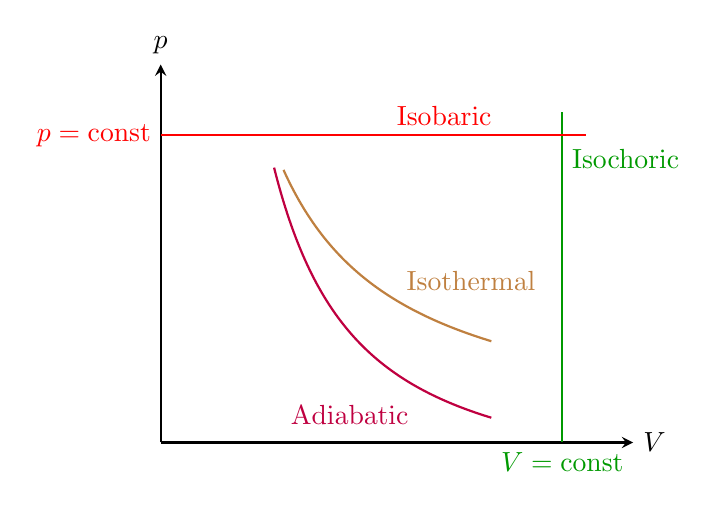
\begin{tikzpicture}[>=stealth, scale=1.2]
    % Tengelyek feketével, nyilakkal
    \draw[->, thick] (0,0) -- (5,0) node[right] {$V$};
    \draw[->, thick] (0,0) -- (0,4) node[above] {$p$};

    % Izochor (Zöld függőleges vonal)
    \draw[green!60!black, thick] (4.25, 0) -- (4.25, 3.5);
    \node[green!60!black, below] at (4.25, 0) {$V = \text{const}$};
    \node[green!60!black, right] at (4.25, 3) {Isochoric};

    % Izobár (Vörös vízszintes vonal)
    \draw[red, thick] (0, 3.25) -- (4.5, 3.25);
    \node[red, left] at (0, 3.25) {$p = \text{const}$};
    \node[red, above] at (3, 3.25) {Isobaric};

    % Metszéspont meghatározása a görbék indításához
    % (1.5, 2.5) a metszéspont
    
    % Izoterma (Barna görbe: p = k/V)
    % Úgy rajzoljuk, hogy átmenjen a metszésponton (1.5 * 2.5 = 3.75)
    \draw[brown, thick, domain=1.3:3.5, samples=100] plot (\x, {3.75/\x});
    \node[brown, above right] at (2.5, 1.5) {Isothermal};

    % Adiabata (Lila görbe: p = k/V^gamma)
    % Meredekebb, mint az izoterma. k = 2.5 * 1.5^1.4 ≈ 4.4
    \draw[purple, thick, domain=1.2:3.5, samples=100] plot (\x, {4.4/(\x^1.4)-0.5});
    \node[purple, below] at (2.0, 0.5) {Adiabatic};

\end{tikzpicture}
\end{center}

\end{itemize}

\end{frame}

% ----------------------------------------------------------------------------------------------------------------------------------------

\begin{frame}
%\frametitle{Minden jó, ha a vége jó}

\vfill
\begin{center}
\textbf{\huge The End}

\bigskip
Thank you for your attention!
\end{center}
\vfill
\textbf{Acknowledgements} Thank you for the course materials for Szilárd~ZSÓKA and Zoltán~VARGA.
\end{frame}

\end{document}
